\documentclass[11pt,a4paper,onecolumn,oneside]{tau-class/tau}
\usepackage{fontspec}
\setmainfont{TeX Gyre Termes}
\usepackage{unicode-math}
\setmathfont{TeX Gyre Termes Math}
\usepackage[english]{babel}
\usepackage[UTF8,scheme=plain,fontset=fandol]{ctex}
\setCJKsansfont{FandolHei-Regular.otf}[BoldFont=FandolHei-Bold.otf,ItalicFont=FandolKai-Regular.otf]
\usepackage{xurl}
\renewcommand{\figurename}{图}
\renewcommand{\tablename}{表}
\renewcommand{\refname}{参考文献}
\usepackage{tabularx}
\geometry{margin=22mm,bottom=25mm}
\setlength{\emergencystretch}{2em}
\raggedbottom
\setcounter{topnumber}{2}
\setcounter{bottomnumber}{2}
\setcounter{totalnumber}{4}
\renewcommand{\topfraction}{.85}
\renewcommand{\bottomfraction}{.7}
\renewcommand{\textfraction}{.12}
\renewcommand{\floatpagefraction}{.75}
\definecolor{taucolor}{HTML}{245D4B}
\hypersetup{pdftitle={同类包装食品中，价格与营养和环境表现有何关系？},pdfauthor={食品价格、营养与环境影响项目组}}
\doctype{课程研究报告}
\title{同类包装食品中，价格与营养和环境表现有何关系？}
\author{食品价格、营养与环境影响项目组}
\dates{2026 年 11 月 11 日 | 法国 | R for Data Science}
\footinfo{食品比较}
\organization{课程研究}
\leadauthor{法国 / 2024--2025 年价格}
\theday{2026 年 11 月 11 日}
\renewcommand{\abstractname}{摘要}
\AtBeginDocument{\renewcommand{\abstractname}{摘要}}
\begin{abstract}
同类食品中，较高价格对应怎样的营养和环境表现？我们连接法国 2024--2025 年 Open Prices 报价与 2026 年获取的 Open Food Facts 商品资料，对四类共 598 款商品开展类别内探索性分析。早餐谷物和黑巧克力的价格与两项综合分数呈有利关联，饼干和果汁的关联接近零。黑巧克力的高价同时对应少糖与较高饱和脂肪。583 款价格与两项等级齐全的商品中，562 款存在更便宜且两项等级均不差的同类选项。研究结果支持先按类别与单位价格设预算，再结合等级和成分比较商品。配套 Shiny 仪表板提供图表探索与两商品比较。
\end{abstract}
\keywords{消费者选择，单位价格，营养，环境等级，Shiny}
\AtBeginDocument{
\renewcommand{\figurename}{图}
\renewcommand{\tablename}{表}
\renewcommand{\refname}{参考文献}
\renewcommand{\keywordname}{关键词：}
\captionsetup[figure]{name=图}
\captionsetup[table]{name=表}
}
\begin{document}
\maketitle\thispagestyle{firststyle}
\section{Introduction}
消费者在比较两款同类包装食品时，需要同时考虑价格、营养和环境表现。包装大小不同，整包售价很难直接比较。统一为每公斤或每升的价格后，还需要回答一个问题：价格更高的商品，在营养和环境上通常会有怎样的表现？这个问题也关系到零售商的商品定位，因为价格背后的属性决定了哪些产品值得进一步对标。

现有研究说明，食品价格与可持续性之间的关系会随比较尺度而变化。按每 100 g 和每 100 kcal 比较，可能得到不同的关联\cite{masset2015}。跨国食品研究发现，不同食品组的价格与营养、环境属性呈现不同关系\cite{martinez2025}。商品层面的营养与环境研究也提示，两项表现需要分别观察\cite{clark2022}。这些研究使本项目采用类别内比较，并同时保留综合评分和具体营养成分。

我们选取法国市场的饼干、早餐谷物、黑巧克力和果汁，研究三个问题。\textbf{RQ1}，同类食品中，单位价格与营养分数及成分有什么关系？\textbf{RQ2}，单位价格与环境分数有什么关系？\textbf{RQ3}，在当前样本里，哪些商品能找到价格更低、两项等级均不差的同类选项？前两问用于理解整体趋势，第三问把分析落到具体商品的比较。

\section{Data and Methods}
\subsection{数据来源与样本}
价格来自 Open Prices 的法国门店记录，范围为 2024--2025 年、EUR 计价的条码商品。商品资料来自 2026 年 11 月 2 日获取的 Open Food Facts，包含包装规格、营养成分和两套评分。两份资料按字符型商品条码连接，一条码代表一款商品。

从符合类别、规格和常规报价条件的 3,002 款候选商品中，以固定随机种子 20261102 在四类中各抽取 150 款。两款因净含量缺失或规格冲突被排除，主要比较集为 598 款，连接 1,541 条报价。抽样时保留评分缺失的商品，每项分析按所需字段选择有效样本。四类的等额抽样便于比较类别内关系。
\begin{table}[!ht]\centering\small\caption{四类商品的样本量、价格中位数与等级覆盖。每款商品在类别汇总中具有相同权重。}\begin{tabular}{lrlrrr}
\toprule
类别 & $n$ & 单位 & 中位数 & 营养 $n$ & 环境 $n$ \\
\midrule
饼干 & 149 & EUR/kg & 11.09 & 147 & 148 \\
早餐谷物 & 150 & EUR/kg & 8.27 & 147 & 150 \\
黑巧克力 & 149 & EUR/kg & 25.83 & 146 & 149 \\
果汁 & 150 & EUR/L & 2.85 & 145 & 149 \\
\bottomrule
\end{tabular}
\label{tab:sample}\end{table}

\subsection{价格、营养与环境指标}
饼干、早餐谷物和黑巧克力统一为 EUR/kg，果汁统一为 EUR/L。每款商品取去重后有效非折扣单位报价的中位数，作为代表价格。报价次数和日期保留在商品对比中，供读者判断价格依据。

营养采用 Nutri-Score 2023，等级从 A 到 E，数值分数越低越好。糖、饱和脂肪和膳食纤维按每 100 g 展示，果汁按每 100 ml 展示。环境综合等级从 A+ 到 F，数值分数越高越好。数据检查发现原清洗规则将 16 个有效 F 级当作缺失，我们从同批原始响应恢复这些等级，并与法国地域分数配对。修正后，596 款具有环境等级，583 款同时具有价格与两项等级。

\subsection{分析方法}
我们先检查字段覆盖和价格分布，再用箱线图比较不同等级中的价格，并计算类别内 Spearman 秩相关。$\rho$ 描述价格与另一项数值按高低排序时的关联方向和程度。每个系数使用价格和该指标均完整的商品，表中同时列出有效样本量。价格分布图使用对数坐标，使较宽的价格范围能够清楚显示。

对 RQ3，我们在同类中逐款寻找代表价格严格更低、营养等级与环境等级分别至少持平的商品。两套等级各按自身顺序比较。商品对比继续展示配方和包装，帮助判断备选是否适合相同用途。

敏感性分析依次采用含折扣价格、保留重复报价的价格、分年价格和每 100 kcal 价格，并单独查看至少有两条常规报价的商品。替代口径在同一批商品上与主口径配对比较。AGRIBALYSE 3.2 碳估算按标准参考食品汇总，保留 kg CO$_2$e/kg 食品的功能单位。

\section{Results}
\subsection{价格与评分的关系随食品类别变化}
早餐谷物和黑巧克力呈现价格较高时营养分数较低、环境分数较高的倾向。饼干和果汁的两项相关均接近零，价格排序对评分排序提供的提示很少。表~\ref{tab:associations} 回答 RQ1 和 RQ2，显示这种类别差异。
\begin{table}[!ht]\centering\scriptsize\caption{类别内价格与综合分数的 Spearman 相关。营养分数越低越好，环境分数越高越好。每项系数使用自己的有效样本。}\begin{tabular}{lrrrr}
\toprule
类别 & 营养 $n$ & $\rho$ 价格--营养 & 环境 $n$ & $\rho$ 价格--环境 \\
\midrule
饼干 & 147 & 0.022 & 148 & 0.030 \\
早餐谷物 & 147 & -0.196 & 150 & 0.307 \\
黑巧克力 & 146 & -0.271 & 149 & 0.243 \\
果汁 & 145 & 0.025 & 149 & 0.035 \\
\bottomrule
\end{tabular}
\label{tab:associations}\end{table}

\begin{figure}[!htbp]\centering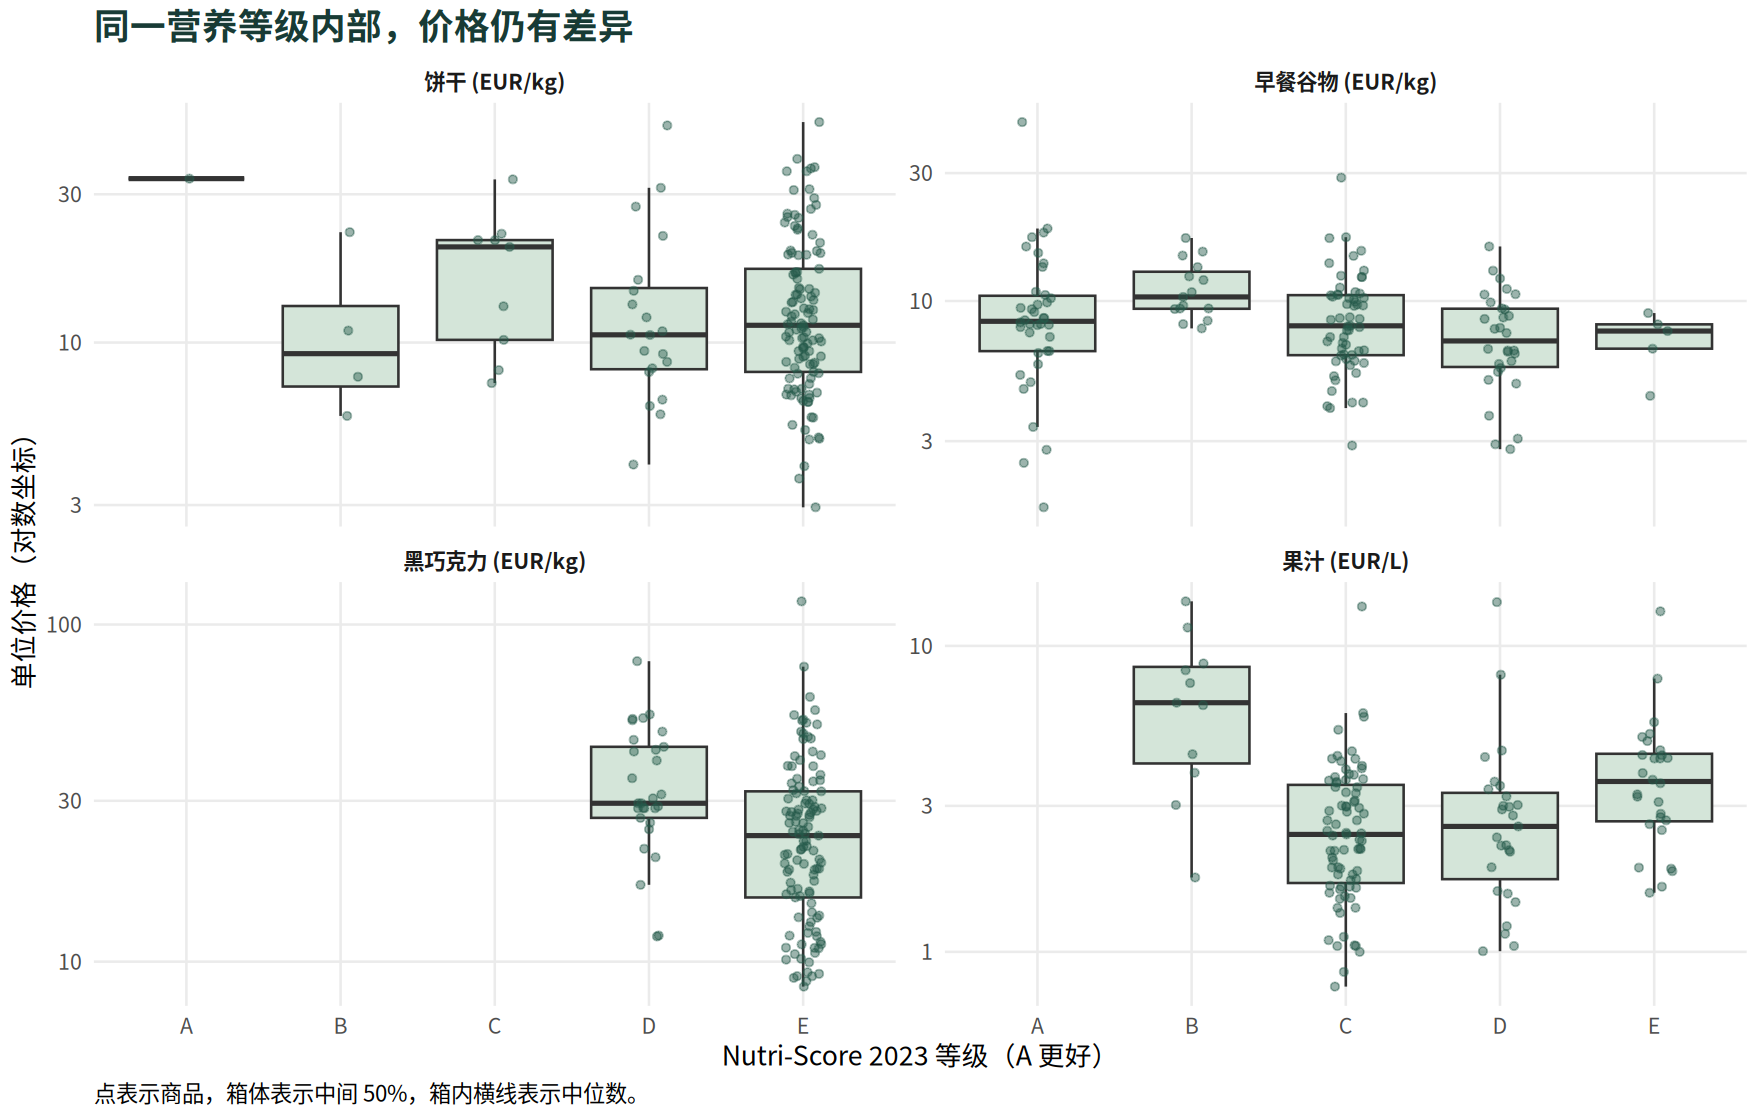
\includegraphics[width=\linewidth,height=.32\textheight,keepaspectratio]{generated/figures/zh/price_nutrition.png}\caption{同一营养等级中的商品仍有价格差异。横轴为 Nutri-Score 等级，纵轴为对数单位价格。每点是一款商品，箱体显示中间 50\% 的价格，中线为中位数。四个面板分别显示四类食品，采用各自的价格尺度。}\label{fig:nutrition}\end{figure}

图~\ref{fig:nutrition} 补充了相关系数之外的分布信息。饼干样本的 147 款有效营养等级中，113 款为 E，A 级只有一款。黑巧克力仅有 D、E 两个等级。这些集中分布使具体成分成为进一步比较商品的重要依据。

\begin{figure}[!htbp]\centering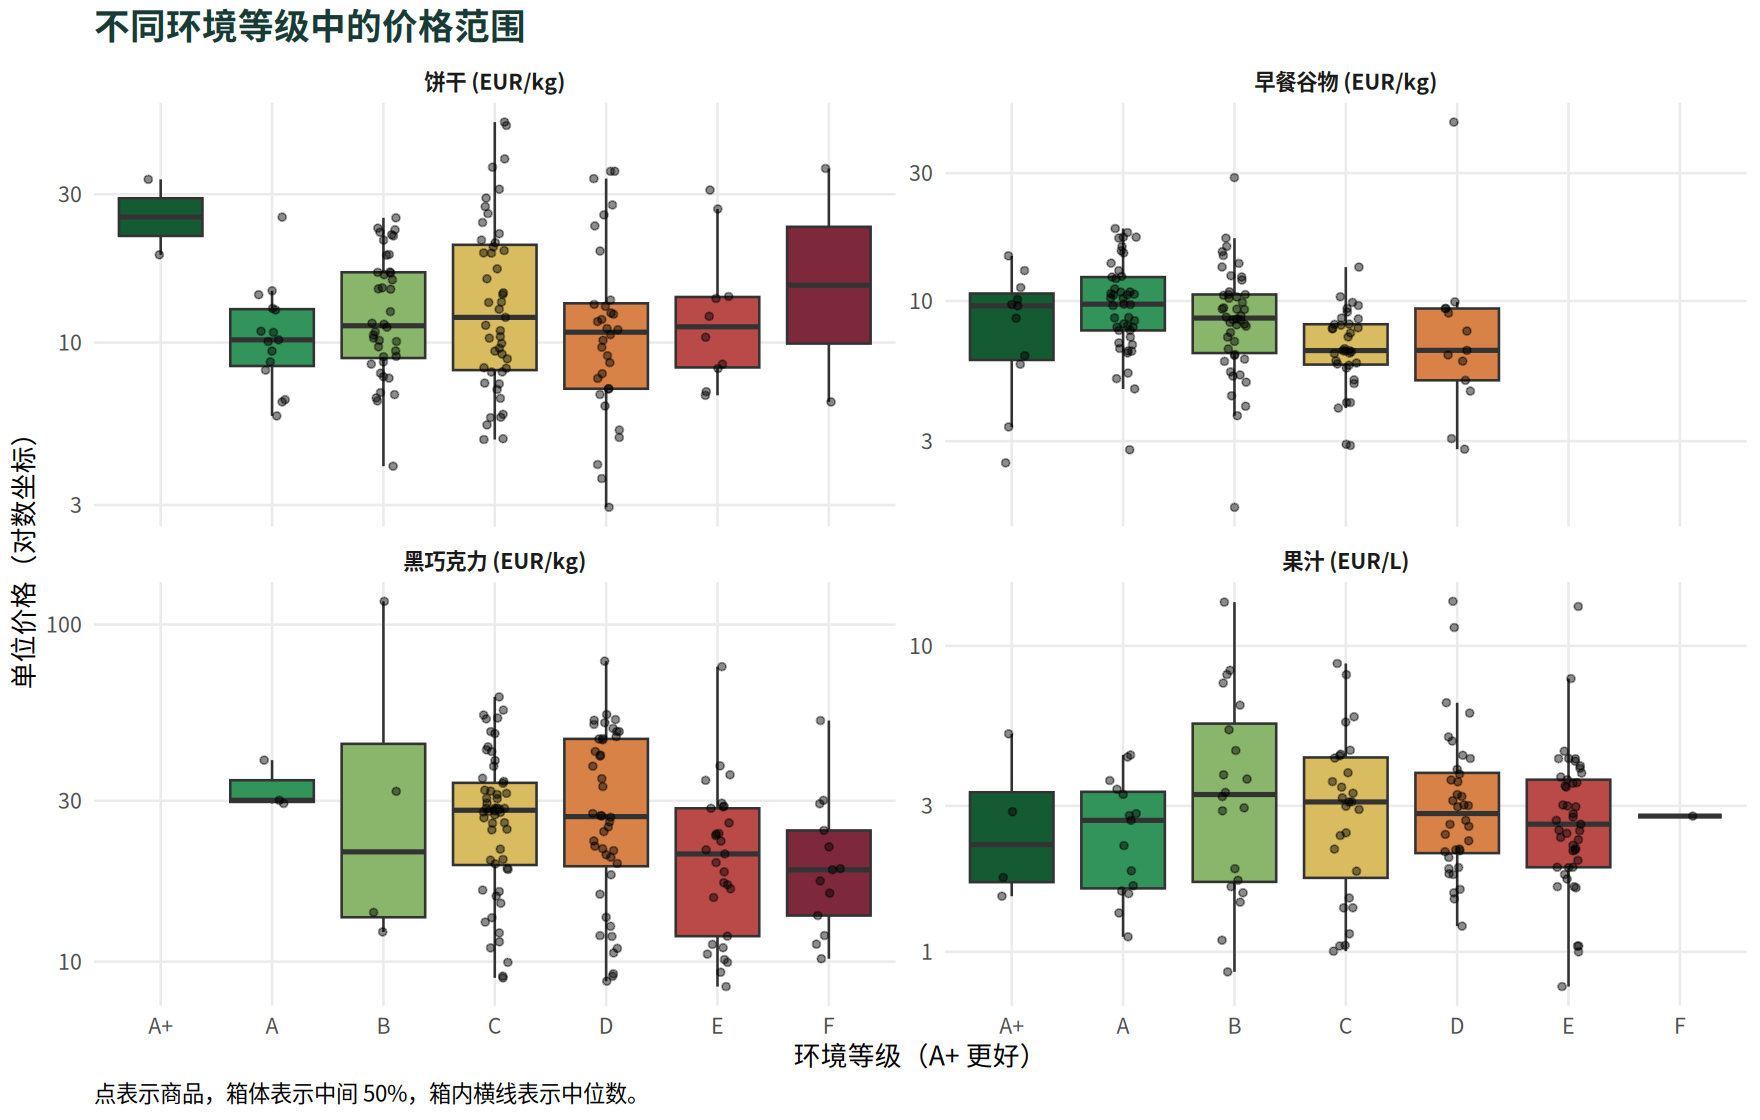
\includegraphics[width=\linewidth,height=.32\textheight,keepaspectratio]{generated/figures/zh/price_environment.png}\caption{不同环境等级中的历史单位价格分布。横轴从较好的 A+ 排到 F，纵轴为对数单位价格。每点是一款商品，箱体与中线分别表示中间 50\% 和中位数。表~\ref{tab:associations} 的相关系数采用对应的数值环境分数。}\label{fig:environment}\end{figure}

环境分数与价格的相关在早餐谷物中为 $\rho=0.307$，黑巧克力为 $0.243$。这两类中，价格较高与环境分数较高有一定关联。饼干与果汁的系数分别为 $0.030$ 和 $0.035$。图~\ref{fig:environment} 展示等级内部的价格范围，读者可以在一个等级中继续寻找价格不同的商品。

\subsection{黑巧克力呈现糖与饱和脂肪的取舍}
在 148 款糖数值完整的黑巧克力中，价格与糖含量的相关为 $\rho=-0.456$。在 148 款饱和脂肪数值完整的商品中，对应相关为 $\rho=0.401$。较贵的商品往往糖更少，同时饱和脂肪更多。图~\ref{fig:composition} 将这两项结果放在一起，说明解释商品差异时需要同时读两项成分。
\begin{figure}[!htbp]\centering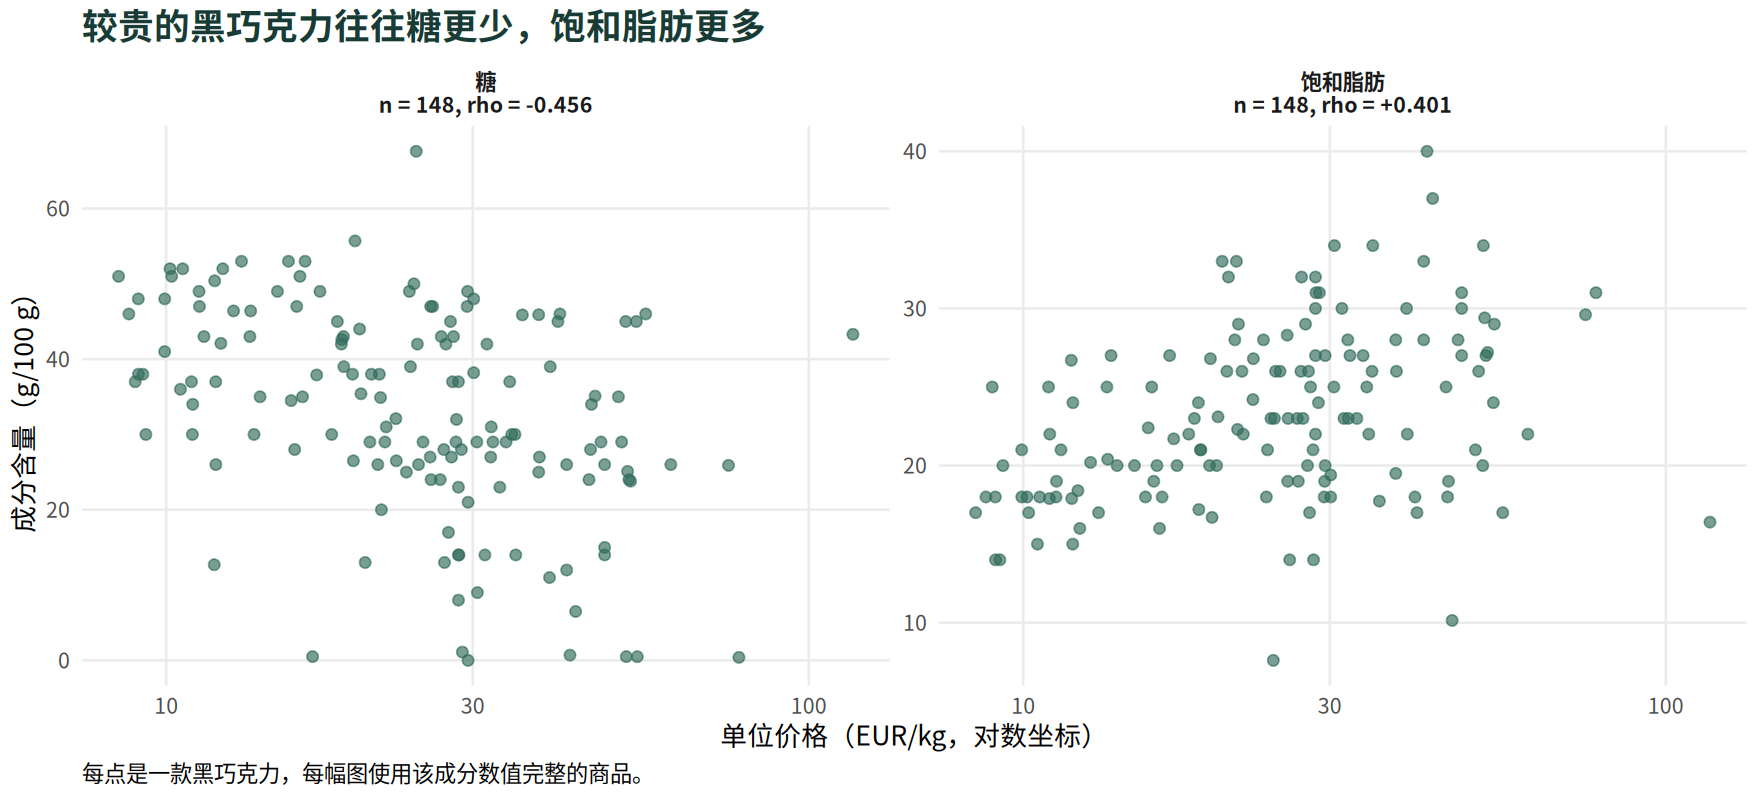
\includegraphics[width=\linewidth,height=.30\textheight,keepaspectratio]{generated/figures/zh/chocolate_composition.png}\caption{黑巧克力的两项营养成分随价格呈现相反方向。横轴为对数单位价格，纵轴为每 100 g 的成分含量，每点是一款商品。左图的糖与价格呈负关联，右图的饱和脂肪与价格呈正关联。}\label{fig:composition}\end{figure}

\subsection{大多数联合样本商品存在低价备选}
583 款三项指标齐全的商品中，562 款（96.4\%）能在同类样本中找到至少一个更便宜、两项等级均不差的选项。各类占比为 95.2\%--98.6\%（表~\ref{tab:candidates}）。这个结果回答 RQ3，说明逐款比较可以发现平均趋势之外的具体选择。
\begin{table}[!ht]\centering\small\caption{具有低价备选的商品数。每款商品只要存在至少一个符合规则的选项，就计入一次。}\begin{tabular}{lrrrr}
\toprule
类别 & 联合 $n$ & 有候选商品 & 占比 & 非劣势商品 \\
\midrule
饼干 & 146 & 139 & 95.2\% & 7 \\
早餐谷物 & 147 & 145 & 98.6\% & 2 \\
黑巧克力 & 146 & 139 & 95.2\% & 7 \\
果汁 & 144 & 139 & 96.5\% & 5 \\
\bottomrule
\end{tabular}
\label{tab:candidates}\end{table}

\begin{table}[!ht]\centering\small\caption{两款饼干的实例。B 的历史单位价低 45.7\%，营养等级相同，环境等级更好。}\begin{tabular}{lrr}
\toprule
指标 & 商品 A & 候选 B \\
\midrule
条码 & 3350031923081 & 3410280136257 \\
单位价格 (EUR/kg) & 7.36 & 4.00 \\
营养等级 & E & E \\
环境等级 & C & B \\
\bottomrule
\end{tabular}
\label{tab:pair}\end{table}
表~\ref{tab:pair} 的 A 为 Galettes bretonnes pur beurre，B 为 Petit beurre 200g。A 的代表价格是 EUR 7.36/kg，B 是 EUR 4.00/kg，差 EUR 3.36/kg。两款营养等级同为 E，环境等级分别为 C 和 B。A 有两条常规报价，B 的一条报价来自 2024 年 1 月 10 日。这组结果使 B 成为值得进一步核对配方、规格和当前门店价格的备选。

\subsection{价格口径与记录数量影响解释}
纳入折扣价格改变了 15 款商品的代表价格，保留重复报价也改变了 15 款。仅保留多条常规报价的商品时，早餐谷物和黑巧克力的两项关联保持原来的方向，饼干和果汁仍接近零。按每 100 kcal 计价后，同一批果汁的价格--营养分数相关由 $0.041$ 变为 $-0.153$。每升与每单位能量回答不同的比较问题，主分析因此采用与购买规格一致的 kg/L 口径。

\section{Discussion}
三项结果共同支持按类别开展商品比较。早餐谷物和黑巧克力的价格包含一定的营养与环境评分信息，而饼干和果汁需要直接读取属性。黑巧克力进一步说明，综合分数较好的方向仍可能伴随成分之间的取舍。低价备选分析则将这些整体关系落实到两款商品，让读者按自己的用途作判断。

这些发现与文献对食品组差异和功能单位的重视相呼应\cite{masset2015,martinez2025}。现有八篇来源综述还提供了食品可持续性、价格变化及绿色溢价的背景\cite{masset2014,hoenink2024,nakavachara2025,clark2022,desiderio2026,bai2025}。本项目以四类包装食品展示这种差异，并将结果转成可以交互检查的商品比较。

价格记录来自社群贡献，四类等额样本描述的是本次收集到的商品。291 款只有一条常规报价，历史报价与 2026 年的商品资料也存在时间差。较粗的等级增加了两款商品同级的可能性，口味和用途仍会影响替代选择。594 款具有 AGRIBALYSE 3.2 碳估算，其中 150 款谷物只有四个不同碳值，反映标准参考食品的共享映射。上述特点界定了结果的适用范围，后续可补充当前门店价格并细分配方和用途。

\section{Shiny Dashboard}
Shiny 沿用研究的三个问题。类别概览显示价格分布，并分别报告该类的营养和环境关联。探索页将问题、坐标含义和当前筛选结果放在同一张图旁，筛选改变后重新计算有效样本与关联。黑巧克力可在糖和饱和脂肪间切换，商品比较页则展开两款商品的价格与成分差异。

消费者用类别价格设定预算，再挑选适合自己的备选。供应商或产品分析师用同一份结果寻找零售价格与商品属性的对标对象。两种角色共用数据，行动说明随角色调整。课堂试用可以记录选品任务完成率与耗时，了解图表说明是否帮助使用者解释自己的选择。进一步的商业分析还需要当前价格、成本与客户需求资料。

\section{Conclusion}
在这四类法国包装食品中，价格与营养和环境表现的关系随类别变化。早餐谷物和黑巧克力呈现价格较高、综合分数较好的倾向，饼干和果汁的关联接近零。黑巧克力的少糖与较高饱和脂肪同时出现，说明具体成分决定了消费者需要权衡什么。583 款联合样本中，562 款有更便宜且两项等级均不差的同类选项。

\textbf{我们的判断是，先用单位价格设定预算，再用等级和成分比较具体商品。} Shiny 将这个顺序落实为类别选择、图表探索和两商品比较，帮助使用者解释多花的钱对应哪些属性，以及低价备选是否适合自己的用途。

\appendix
\section{复现、来源与协助说明}
R 分析源文件为 \nolinkurl{R/10_eda.R}，完整 notebook 为 \nolinkurl{notebooks/step4_eda.Rmd}。四份数值表从 \nolinkurl{outputs/step4/tables/} 生成。报告图由 \nolinkurl{scripts/build_report_figures.R} 绘制，中英文共用数据与绘图规则。运行 \nolinkurl{scripts/run_step4.ps1} 重建分析，\nolinkurl{scripts/build_report.ps1} 编译报告，\nolinkurl{scripts/run_shiny.ps1} 启动应用。

价格与商品数据库来自 Open Prices / Open Food Facts contributors，许可和处理记录见 \nolinkurl{data/README.md}。项目使用 Tau-class 2.6.0（Guillermo Jimenez，CC BY 4.0）。Shiny 的场景插图由 AI 生成，来源记录见 \nolinkurl{reports/assets/provenance.json}。AI 参与代码生成、报告起草和检查。成员署名贡献、个人反思与课堂反馈由小组在课程提交时补充。Masset（2014）和 Bai（2025）的综述提炼依据摘要，阅读范围记录在文献综述中。
\begin{thebibliography}{9}\small
\bibitem{masset2014} Masset, G., et al. (2014). Identifying sustainable foods: The relationship between environmental impact, nutritional quality, and prices of foods representative of the French diet. \textit{JAND, 114}, 862--869. \url{https://doi.org/10.1016/j.jand.2014.02.002}.
\bibitem{masset2015} Masset, G., Vieux, F., \& Darmon, N. (2015). Which functional unit to identify sustainable foods? \textit{Public Health Nutrition, 18}, 2488--2497. \url{https://doi.org/10.1017/S1368980015000579}.
\bibitem{hoenink2024} Hoenink, J. C., et al. (2024). Changes in UK price disparities between healthy and less healthy foods over 10 years. \textit{Appetite, 197}, 107290. \url{https://doi.org/10.1016/j.appet.2024.107290}.
\bibitem{martinez2025} Martinez, E. M., et al. (2025). Retail prices, environmental footprints, and nutritional profiles of commonly sold retail food items in 181 countries. \textit{AJCN, 122}, 1265--1274. \url{https://doi.org/10.1016/j.ajcnut.2025.08.002}.
\bibitem{nakavachara2025} Nakavachara, V., et al. (2025). The green premium puzzle. Preprint, v1. \url{https://arxiv.org/abs/2507.10333v1}.
\bibitem{clark2022} Clark, M., et al. (2022). Estimating the environmental impacts of 57,000 food products. \textit{PNAS, 119}, e2120584119. \url{https://doi.org/10.1073/pnas.2120584119}.
\bibitem{desiderio2026} Desiderio, A., et al. (2026). Mapping regional disparities in discounted grocery products. \textit{npj Science of Food, 10}, 112. \url{https://doi.org/10.1038/s41538-026-00764-0}.
\bibitem{bai2025} Bai, Y., et al. (2025). Environmental impacts and monetary costs of healthy diets worldwide. \textit{Nature Food, 6}, 1176--1185. \url{https://doi.org/10.1038/s43016-025-01270-4}.
\end{thebibliography}
\end{document}
